%%%%%%%%%%%%%%%%%%%%%%%%%%%%%%%%%%%%%%%%%%%%%%%%%%%%%%%%%%%%%%%%%%
%%%%%%%%%%%%%%%%%%%%%%%%%%%%%%%%%%%%%%%%%%%%%%%%%%%%%%%%%%%%%%%%%%
%Packages
\documentclass[10pt, a4paper]{article}
\usepackage[top=3cm, bottom=4cm, left=3.5cm, right=3.5cm]{geometry}
\usepackage{amsmath,amsthm,amsfonts,amssymb,amscd, fancyhdr, color, comment, graphicx, environ}
\usepackage{float}
\usepackage{mathrsfs}
\usepackage[math-style=ISO]{unicode-math}
\setmathfont{TeX Gyre Termes Math}
\usepackage{lastpage}
\usepackage[dvipsnames]{xcolor}
\usepackage[framemethod=TikZ]{mdframed}
\usepackage{enumerate}
\usepackage[shortlabels]{enumitem}
\usepackage{fancyhdr}
\usepackage{indentfirst}
\usepackage{listings}
\usepackage{sectsty}
\usepackage{thmtools}
\usepackage{shadethm}
\usepackage{hyperref}
\usepackage{setspace}
\hypersetup{
    colorlinks=true,
    linkcolor=blue,
    filecolor=magenta,      
    urlcolor=blue,
}
\usepackage[makeroom]{cancel}
\usepackage[utf8]{inputenc}
\usepackage[T1]{fontenc}
\usepackage{hyperref}
\hypersetup{colorlinks=true, linkcolor=blue, filecolor=magenta, urlcolor=cyan,}
\urlstyle{same}
\usepackage{amsmath}
\usepackage{amsfonts}
\usepackage{amssymb}
\usepackage[version=4]{mhchem}
\usepackage{stmaryrd}
\usepackage{graphicx}
\usepackage{subcaption}
\usepackage[export]{adjustbox}
\graphicspath{ {./images/} }
\usepackage{listings}
%%%%%%%%%%%%%%%%%%%%%%%%%%%%%%%%%%%%%%%%%%%%%%%%%%%%%%%%%%%%%%%%%%
%%%%%%%%%%%%%%%%%%%%%%%%%%%%%%%%%%%%%%%%%%%%%%%%%%%%%%%%%%%%%%%%%%
%Environment setup
\mdfsetup{skipabove=\topskip,skipbelow=\topskip}
\newrobustcmd\ExampleText{%
An \textit{inhomogeneous linear} differential equation has the form
\begin{align}
L[v ] = f,
\end{align}
where $L$ is a linear differential operator, $v$ is the dependent
variable, and $f$ is a given non−zero function of the independent
variables alone.
}
\mdfdefinestyle{theoremstyle}{%
linecolor=black,linewidth=1pt,%
frametitlerule=true,%
frametitlebackgroundcolor=gray!20,
innertopmargin=\topskip,
}
\mdtheorem[style=theoremstyle]{Problem}{Problem}
\newenvironment{Solution}{\textbf{Solution.}}

\definecolor{codegreen}{rgb}{0,0.6,0}
\definecolor{codegray}{rgb}{0.5,0.5,0.5}
\definecolor{codepurple}{rgb}{0.58,0,0.82}
\definecolor{backcolour}{rgb}{0.95,0.95,0.92}

\lstdefinestyle{mystyle}{
    backgroundcolor=\color{backcolour},   
    commentstyle=\color{codegreen},
    keywordstyle=\color{magenta},
    numberstyle=\tiny\color{codegray},
    stringstyle=\color{codepurple},
    basicstyle=\ttfamily\footnotesize,
    breakatwhitespace=false,         
    breaklines=true,                 
    captionpos=b,                    
    keepspaces=true,                 
    numbers=left,                    
    numbersep=5pt,                  
    showspaces=false,                
    showstringspaces=false,
    showtabs=false,                  
    tabsize=2
}

\lstset{style=mystyle}
%%%%%%%%%%%%%%%%%%%%%%%%%%%%%%%%%%%%%%%%%%%%%%%%%%%%%%%%%%%%%%%%%%
%%%%%%%%%%%%%%%%%%%%%%%%%%%%%%%%%%%%%%%%%%%%%%%%%%%%%%%%%%%%%%%%%%
%Fill in the appropriate information below
\newcommand{\norm}[1]{\left\lVert#1\right\rVert}     
\newcommand\course{CS5785}                            % <-- course name   
\newcommand\hwnumber{3}                                 % <-- homework number
\newcommand\Information{Arystan Tatishev, Maanas Peri}                        % <-- personal information
%%%%%%%%%%%%%%%%%%%%%%%%%%%%%%%%%%%%%%%%%%%%%%%%%%%%%%%%%%%%%%%%%%
%%%%%%%%%%%%%%%%%%%%%%%%%%%%%%%%%%%%%%%%%%%%%%%%%%%%%%%%%%%%%%%%%%
%Page setup
\pagestyle{fancy}
\headheight 35pt
\lhead{\today}
\rhead{
\includegraphics[width=2.5cm]{logo-ct.png}}
\lfoot{}
\pagenumbering{arabic}
\cfoot{\small\thepage}
\rfoot{}
\headsep 1.2em
\renewcommand{\baselinestretch}{1.25}
%%%%%%%%%%%%%%%%%%%%%%%%%%%%%%%%%%%%%%%%%%%%%%%%%%%%%%%%%%%%%%%%%%
%%%%%%%%%%%%%%%%%%%%%%%%%%%%%%%%%%%%%%%%%%%%%%%%%%%%%%%%%%%%%%%%%%
%Add new commands here
\renewcommand{\labelenumi}{\alph{enumi})}
\newcommand{\Z}{\mathbb Z}
\newcommand{\R}{\mathbb R}
\newcommand{\Q}{\mathbb Q}
\newcommand{\NN}{\mathbb N}
\newcommand{\PP}{\mathbb P}
\DeclareMathOperator{\Mod}{Mod} 
\renewcommand\lstlistingname{Algorithm}
\renewcommand\lstlistlistingname{Algorithms}
\def\lstlistingautorefname{Alg.}
\newtheorem*{theorem}{Theorem}
\newtheorem*{lemma}{Lemma}
\newtheorem{case}{Case}
\newcommand{\assign}{:=}
\newcommand{\infixiff}{\text{ iff }}
\newcommand{\nobracket}{}
\newcommand{\backassign}{=:}
\newcommand{\tmmathbf}[1]{\ensuremath{\boldsymbol{#1}}}
\newcommand{\tmop}[1]{\ensuremath{\operatorname{#1}}}
\newcommand{\tmtextbf}[1]{\text{{\bfseries{#1}}}}
\newcommand{\tmtextit}[1]{\text{{\itshape{#1}}}}

\newenvironment{itemizedot}{\begin{itemize} \renewcommand{\labelitemi}{$\bullet$}\renewcommand{\labelitemii}{$\bullet$}\renewcommand{\labelitemiii}{$\bullet$}\renewcommand{\labelitemiv}{$\bullet$}}{\end{itemize}}
\catcode`\<=\active \def<{
\fontencoding{T1}\selectfont\symbol{60}\fontencoding{\encodingdefault}}
\catcode`\>=\active \def>{
\fontencoding{T1}\selectfont\symbol{62}\fontencoding{\encodingdefault}}
\catcode`\<=\active \def<{
\fontencoding{T1}\selectfont\symbol{60}\fontencoding{\encodingdefault}}

%%%%%%%%%%%%%%%%%%%%%%%%%%%%%%%%%%%%%%%%%%%%%%%%%%%%%%%%%%%%%%%%%%
%%%%%%%%%%%%%%%%%%%%%%%%%%%%%%%%%%%%%%%%%%%%%%%%%%%%%%%%%%%%%%%%%%
%Begin now!



\begin{document}

\begin{titlepage}
    \begin{center}
        \vspace*{3cm}
            
        \Huge
        \textbf{Assignment}
            
        \vspace{1cm}
        \huge
        Homework \hwnumber
            
        \vspace{1.5cm}
        \Large
            
        \textbf{\Information}                      % <-- author
        
            
        \vfill
        
        A \course \ Homework Assignment
            
        \vspace{1cm}
            
        
\includegraphics[width=0.4\textwidth]{logo-ct.png}
        \\
        
        \Large
        
        \today
            
    \end{center}
\end{titlepage}

%%%%%%%%%%%%%%%%%%%%%%%%%%%%%%%%%%%%%%%%%%%%%%%%%%%%%%%%%%%%%%%%%%
%%%%%%%%%%%%%%%%%%%%%%%%%%%%%%%%%%%%%%%%%%%%%%%%%%%%%%%%%%%%%%%%%%
%Start the assignment now
%%%%%%%%%%%%%%%%%%%%%%%%%%%%%%%%%%%%%%%%%%%%%%%%%%%%%%%%%%%%%%%%%%
%New problem
\newpage
\section*{Programming Exercises}
\section{Eigenface for face recognition. (45 pts)}
In this problem, you will implement several machine learning techniques from the class to perform classification on text data. Throughout the problem, we will be working on the NLP with Disaster Tweets Kaggle competition, where the task is to predict whether or not a tweet is about a real disaster.

\begin{Problem*}[(a) (2 pts) Download The Face Dataset and unzip faces .zip]
You will find a folder called images which contains all the training and test images; train.txt and test.txt specifies the training set and test (validation) set split respectively, each line gives an image path and the corresponding label.
\end{Problem*}

\begin{Problem*}[(b) (2 pts) Load the training set into a matrix $\mathbf{X}$:]
There are 540 training images in total, each has $50 \times 50$ pixels that need to be concatenated into a 2500 -dimensional vector. So the size of $\mathbf{X}$ should be $540 \times 2500$, where each row is a flattened face image. Pick a face image from $\mathbf{X}$ and display that image in grayscale. Do the same thing for the test set. The size of matrix $\mathbf{X}_{\text {test }}$ for the test set should be $100 \times 2500$.
\end{Problem*}

\begin{Solution}
\begin{lstlisting}[language=Python]
train_labels, train_data = [], []
for line in open('/content/faces/train.txt'):
    im = imageio.imread(line.strip().split()[0])
    train_data.append(im.reshape(2500,))
    train_labels.append(line.strip().split()[1])

train_data, train_labels = np.array(train_data, dtype=float), np.array(train_labels, dtype=int)

print(train_labels)

test_data = []
test_labels = []

for line in open('./faces/test.txt'):
    parts = line.strip().split()
    im = imageio.imread(parts[0])
    test_data.append(im.reshape(2500,))
    test_labels.append(int(parts[1]))  # Assuming the labels are integers

test_data = np.array(test_data, dtype=float)
test_labels = np.array(test_labels, dtype=int)

# Train Face
plt.imshow(train_data[10, :].reshape(50, 50), cmap=cm.Greys_r)
plt.show()
# Test Face
plt.imshow(test_data[11, :].reshape(50, 50), cmap=cm.Greys_r)
plt.show()
\end{lstlisting}

\begin{figure}[H]
    \centering
    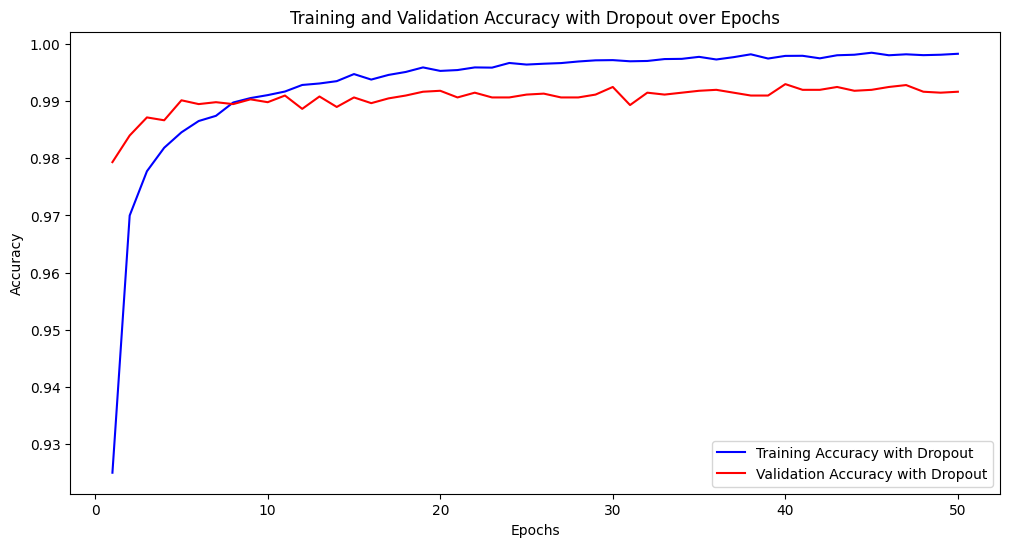
\includegraphics[width=0.5\linewidth]{HW3//images/image9.png}
    \caption{Train Data Image}
    \label{fig:enter-label}
\end{figure}

\begin{figure}[H]
    \centering
    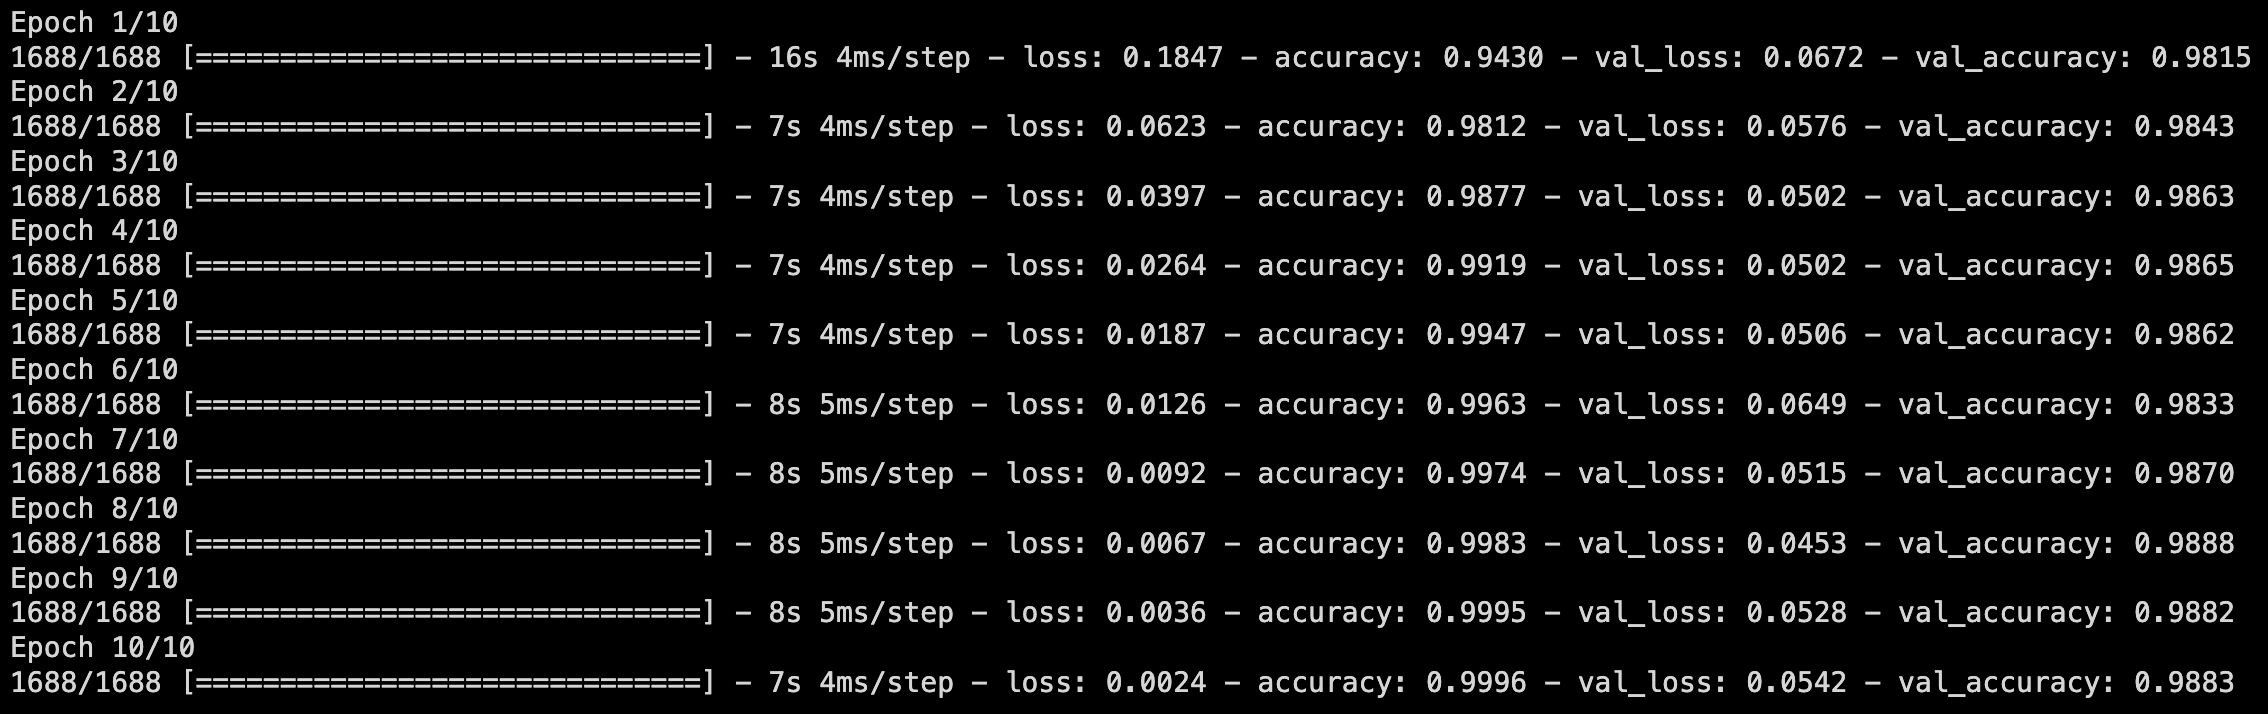
\includegraphics[width=0.5\linewidth]{HW3//images/image10.png}
    \caption{Test Data Image}
    \label{fig:enter-label}
\end{figure}

\end{Solution}

\begin{Problem*}[(c) (3 pts) Average Face. ]
Compute the average face $\mu$ from the whole training set by summing up every row in $\mathbf{X}$ then dividing by the number of faces. Display the average face as a grayscale image.
\end{Problem*}

\begin{Solution}
\begin{lstlisting}[language=Python]
average_face = np.mean(train_data, axis=0)
# Display the average face
plt.imshow(average_face.reshape(50, 50), cmap=cm.Greys_r)
plt.show()
\end{lstlisting}

\begin{figure}[H]
    \centering
    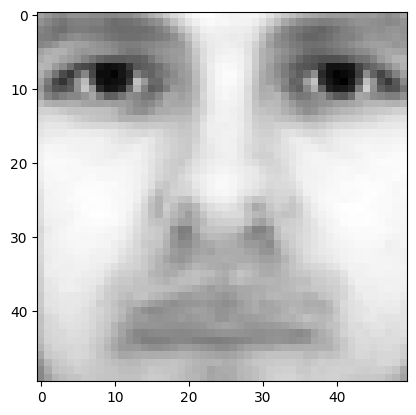
\includegraphics[width=0.5\linewidth]{HW3//images/image2.png}
    \caption{Average Face}
    \label{fig:enter-label}
\end{figure}

\end{Solution}

\begin{Problem*}[(d) (3 pts) Mean Subtraction. ]
Subtract average face $\mu$ from every row in $\mathbf{X}$. That is, $\mathbf{x}_{\mathbf{i}}:=\mathbf{x}_{\mathbf{i}}-$ $\mu$, where $\mathbf{x}_{\mathbf{i}}$ is the $i$-th row of $\mathbf{X}$. Pick a face image after mean subtraction from the new $\mathbf{X}$ and display that image in grayscale. Do the same thing for the test set $\mathbf{X}_{\text {test }}$ using the precomputed average face $\mu$ in (c).
\end{Problem*}

\begin{Solution}
\begin{lstlisting}[language=Python]
train_data_mean_subtracted = train_data - average_face
i = 5
# Display face image after mean subtraction from training data
plt.imshow(train_data_mean_subtracted[i, :].reshape(50, 50), cmap=cm.Greys_r)
plt.title("Training Set: Mean-Subtracted Face Image")
plt.show()

test_data_mean_subtracted = test_data - average_face
# Display the face image after mean subtraction from test data
plt.imshow(test_data_mean_subtracted[i, :].reshape(50, 50), cmap=cm.Greys_r)
plt.title("Test Set: Mean-Subtracted Face Image")
plt.show()
\end{lstlisting}

\begin{figure}[H]
    \centering
    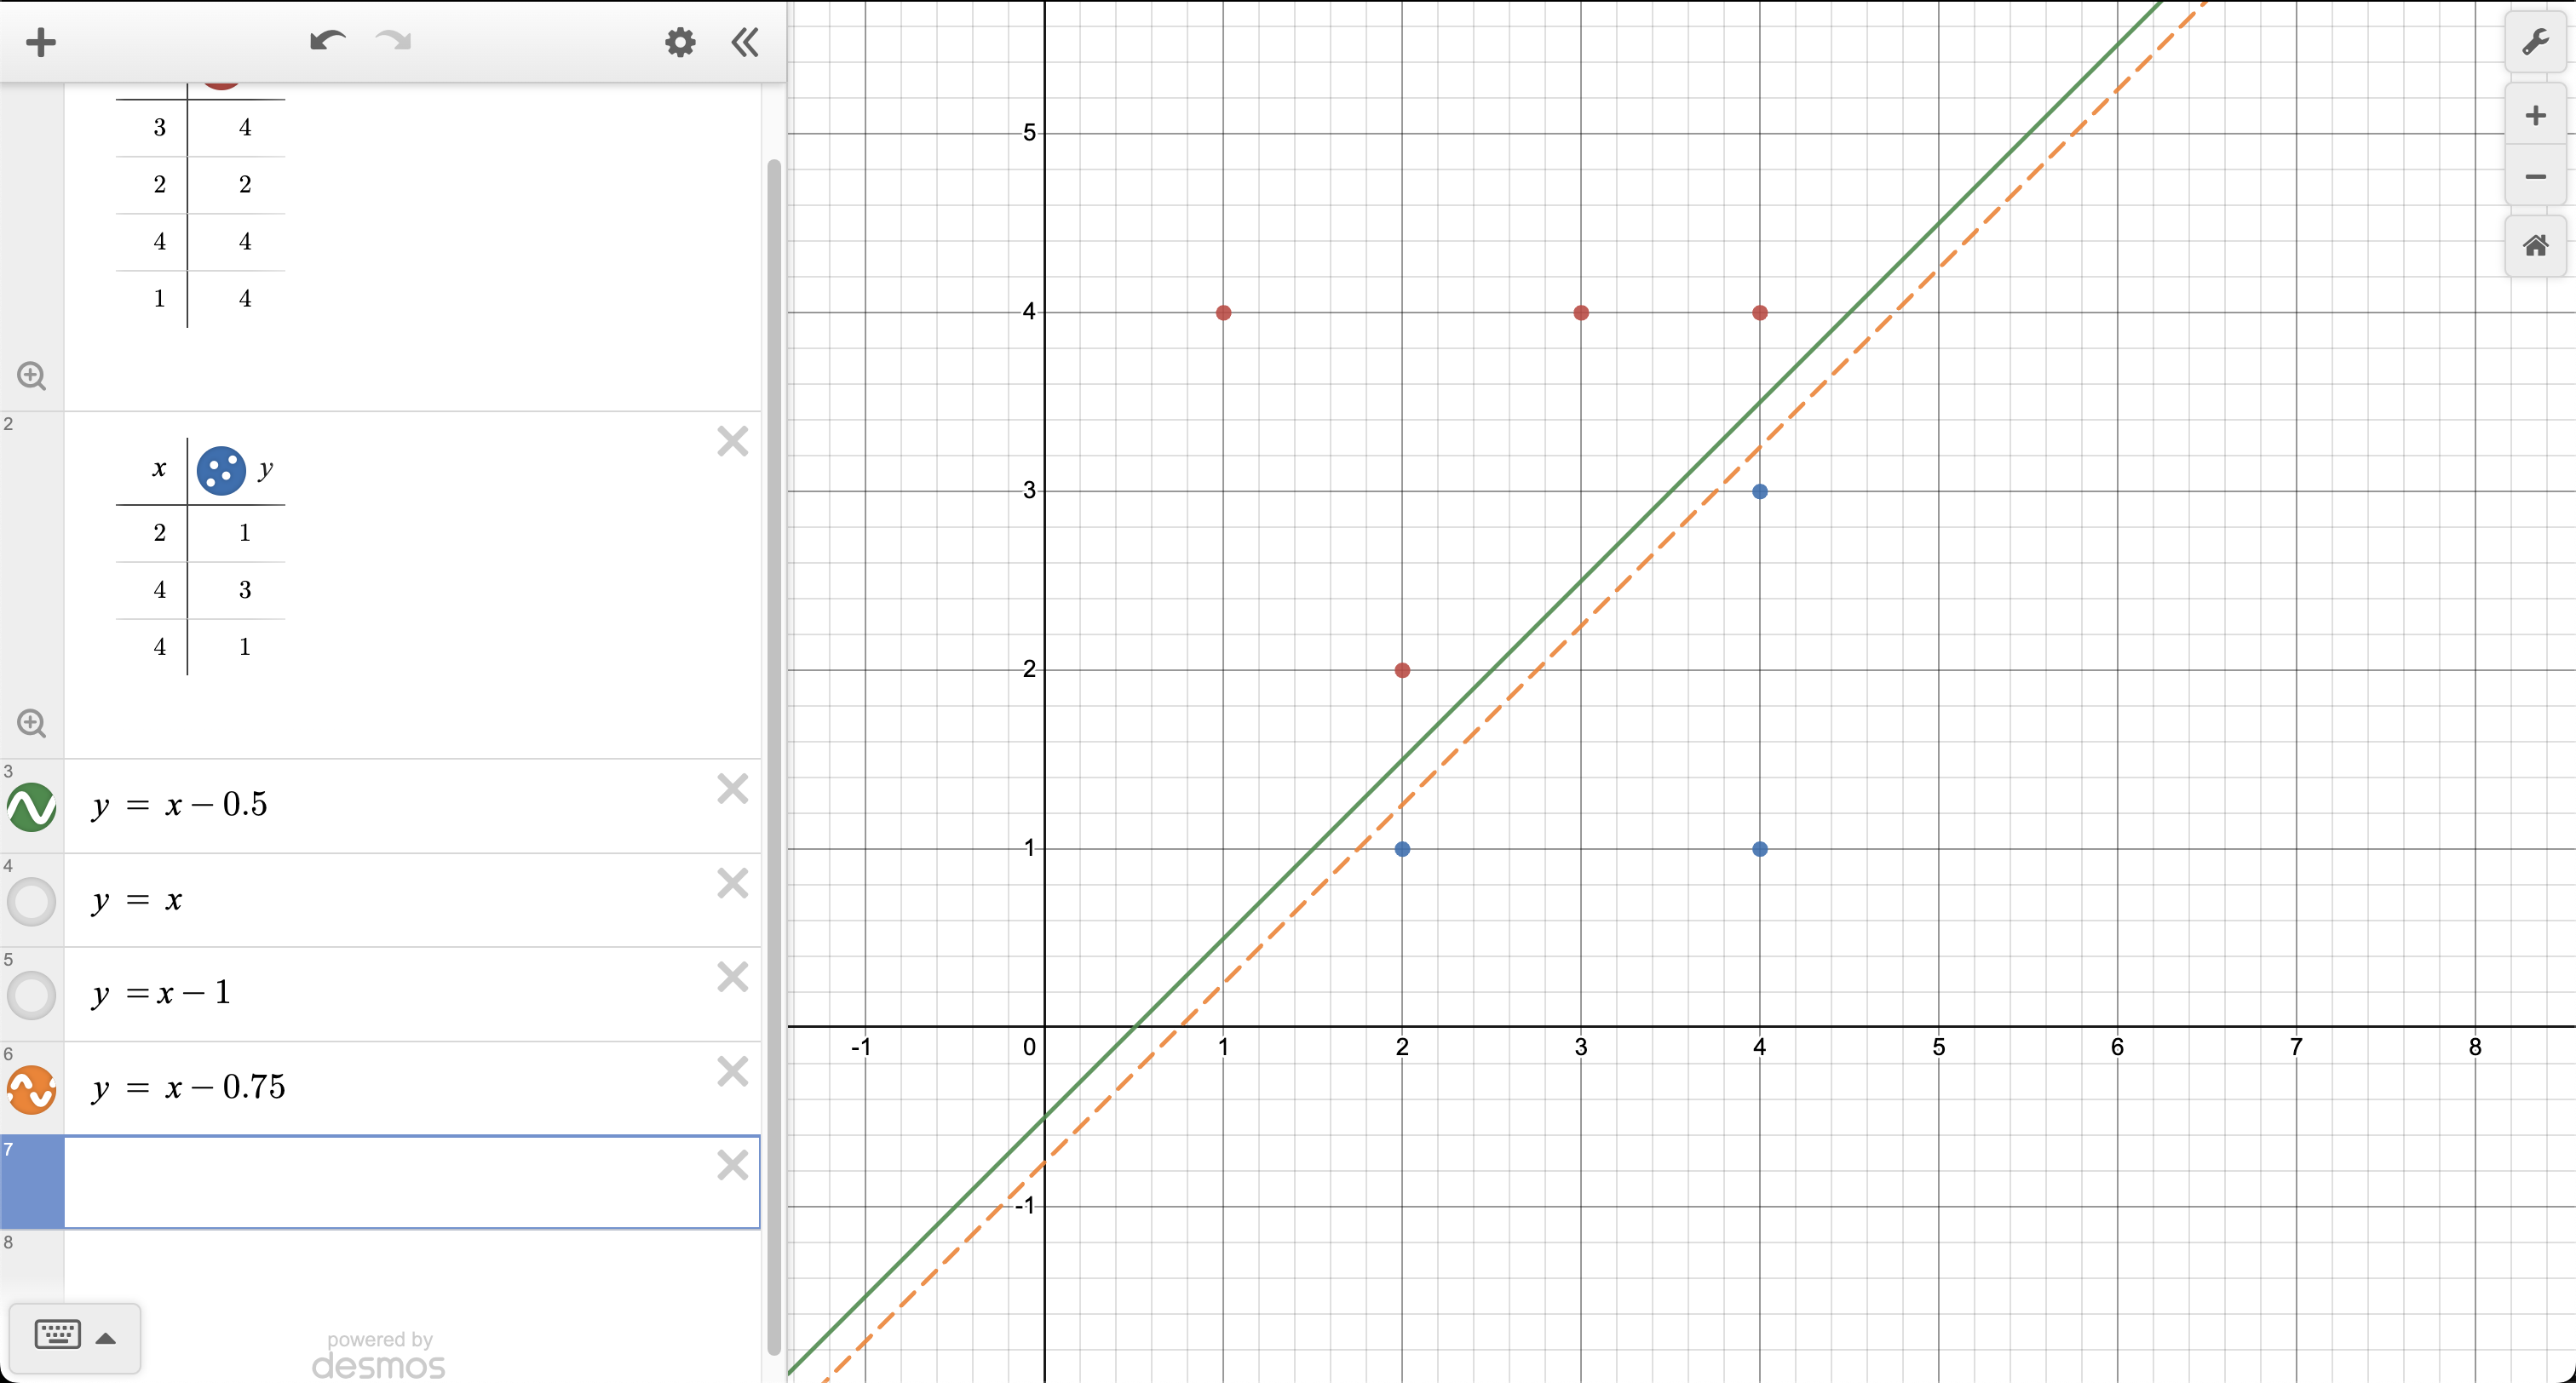
\includegraphics[width=0.5\linewidth]{HW3//images/image3.png}
    \caption{Mean-Subtracted Face Images}
    \label{fig:enter-label}
\end{figure}

\end{Solution}

\begin{Problem*}[(e) (10 pts) Eigenface.]
 Perform eigendecomposition on $\mathbf{X}^{T} \mathbf{X}=\mathbf{V} \Lambda \mathbf{V}^{T}$ to get eigenvectors $\mathbf{V}^{T}$, where each row of $\mathbf{V}^{T}$ has the same dimension as the face image. We refer to $\mathbf{v}_{\mathbf{i}}$, the $i$-th row of $\mathbf{V}^{T}$, as $i$-th eigenface. Display the first 10 eigenfaces as 10 images in grayscale.
\end{Problem*}

\begin{Solution}
\begin{lstlisting}[language=Python]
# Compute covariance matrix
cov_matrix = np.cov(train_data_mean_subtracted, rowvar=False)

# Decompose matrix
eigenvalues, eigenvectors = np.linalg.eigh(cov_matrix)

# Sort eigenvectors
sorted_indices = sorted(range(len(eigenvalues)), key=lambda i: eigenvalues[i], reverse=True)
eigenvectors = np.take(eigenvectors, sorted_indices, axis=1) #sorting eigenvectors by sorted_indices

# Display first 10 eigenfaces
num_eigenfaces_to_display = 10
for i in range(num_eigenfaces_to_display):
    # Get i-th eigenface and reshape to original dimension
    eigenface = eigenvectors[:, i].reshape(50, 50)
    plt.imshow(eigenface, cmap=cm.Greys_r)
    plt.show()
\end{lstlisting}

\begin{figure}[htbp]
    \centering
    % First row
    \begin{subfigure}{0.18\textwidth}
        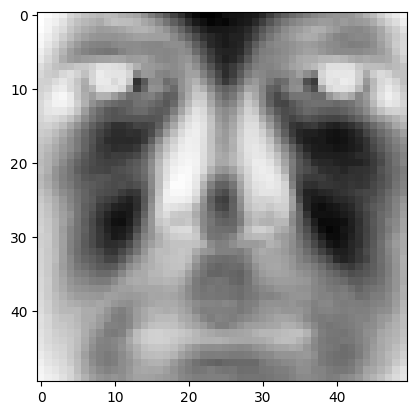
\includegraphics[width=\linewidth]{HW3//images/eigen1.png}
        \caption{}
        \label{fig:sub1}
    \end{subfigure}%
    \hfill
    \begin{subfigure}{0.18\textwidth}
        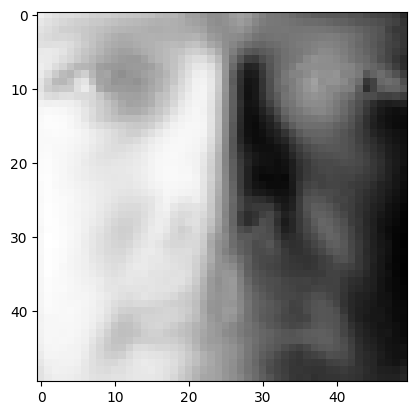
\includegraphics[width=\linewidth]{HW3//images/eigen2.png}
        \caption{}
        \label{fig:sub2}
    \end{subfigure}%
    \hfill
    \begin{subfigure}{0.18\textwidth}
        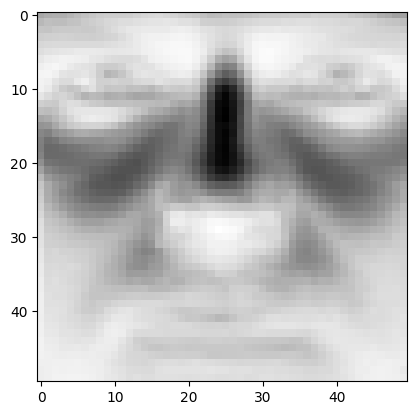
\includegraphics[width=\linewidth]{HW3//images/eigen3.png}
        \caption{}
        \label{fig:sub3}
    \end{subfigure}%
    \hfill
    \begin{subfigure}{0.18\textwidth}
        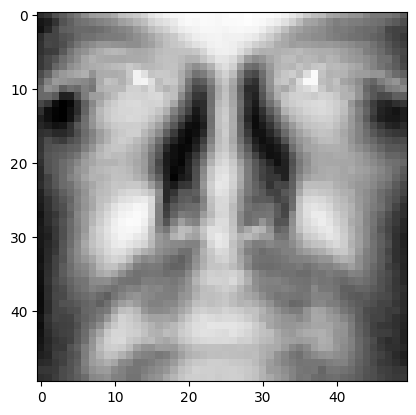
\includegraphics[width=\linewidth]{HW3//images/eigen4.png}
        \caption{}
        \label{fig:sub4}
    \end{subfigure}%
    \hfill
    \begin{subfigure}{0.18\textwidth}
        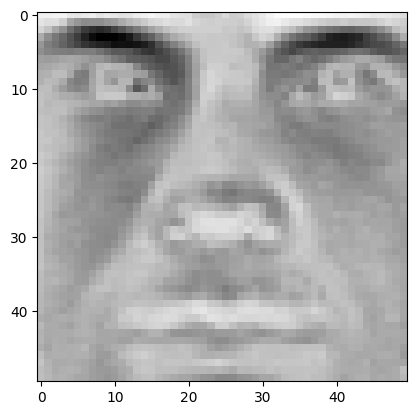
\includegraphics[width=\linewidth]{HW3//images/eigen5.png}
        \caption{}
        \label{fig:sub5}
    \end{subfigure}%

    \vspace{1em} % Gap between rows
    % Second row
    \begin{subfigure}{0.18\textwidth}
        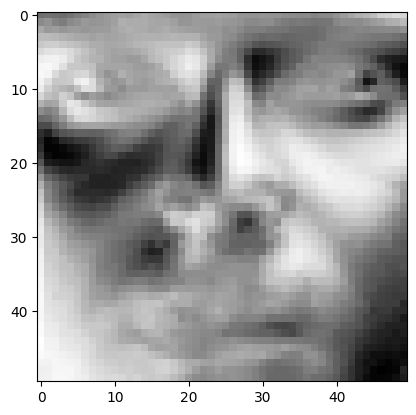
\includegraphics[width=\linewidth]{HW3//images/eigen6.png}
        \caption{}
        \label{fig:sub6}
    \end{subfigure}%
    \hfill
    \begin{subfigure}{0.18\textwidth}
        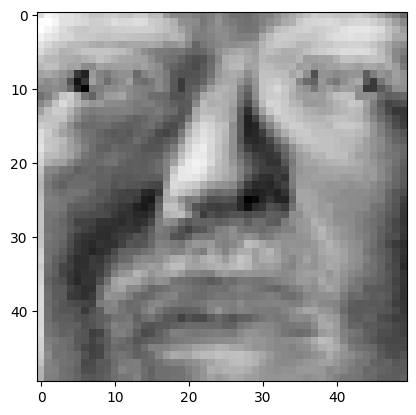
\includegraphics[width=\linewidth]{HW3//images/eigen7.png}
        \caption{}
        \label{fig:sub7}
    \end{subfigure}%
    \hfill
    \begin{subfigure}{0.18\textwidth}
        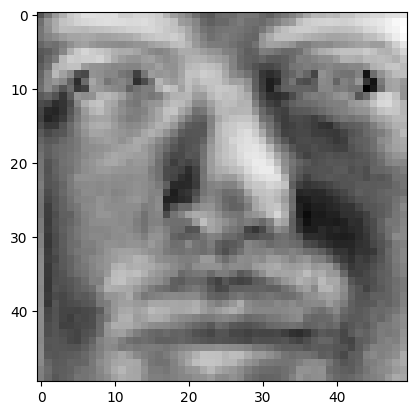
\includegraphics[width=\linewidth]{HW3//images/eigen8.png}
        \caption{}
        \label{fig:sub8}
    \end{subfigure}%
    \hfill
    \begin{subfigure}{0.18\textwidth}
        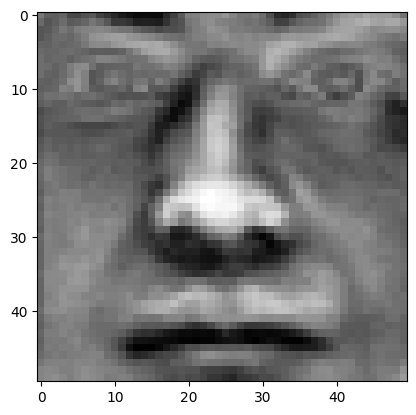
\includegraphics[width=\linewidth]{HW3//images/eigen9.png}
        \caption{}
        \label{fig:sub9}
    \end{subfigure}%
    \hfill
    \begin{subfigure}{0.18\textwidth}
        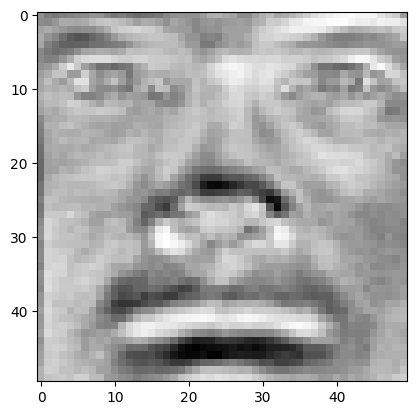
\includegraphics[width=\linewidth]{HW3//images/eigen10.png}
        \caption{}
        \label{fig:sub10}
    \end{subfigure}%

    \caption{Eigenfaces}
    \label{fig:main}
\end{figure}

\end{Solution}

\begin{Problem*}[(f) (10 pts) Eigenface Feature. ]
The top $r$ eigenfaces $\mathbf{V}^{T}[: r:$ : $]=\left\{v_{1}, v_{2}, \ldots, v_{r}\right\}^{T}$ span an $r$-dimensional linear subspace of the original image space called face space, whose origin is the average face $\mu$, and whose axes are the eigenfaces $\left\{\nu_{1}, \nu_{2}, \ldots, \nu_{r}\right\}$. Therefore, using the top $r$ eigenfaces $\left\{v_{1}, \nu_{2}, \ldots, v_{r}\right\}$, we can represent a 2500 -dimensional face image $\mathbf{z}$ as an $r$-dimensional feature vector $\mathbf{f}: \mathbf{f}=\mathbf{V}^{T}[: r::] \mathbf{z}=\left[\nu_{1}, \nu_{2}, \ldots, v_{r}\right]^{T} \mathbf{z}$. Write a function to generate $r$-dimensional feature matrix $\mathbf{F}$ and $\mathbf{F}_{\text {test }}$ for training images $\mathbf{X}$ and test images $\mathbf{X}_{\text {test }}$, respectively (to get $\mathbf{F}$, multiply $\mathbf{X}$ to the transpose of first $r$ rows of $\mathbf{V}^{T}, \mathbf{F}$ should have same number of rows as $\mathbf{X}$ and $r$ columns; similarly for $\mathbf{X}_{\text {test }}$ ).
\end{Problem*}

\begin{Solution}
\begin{lstlisting}[language=Python]
def generate_feature_matrix(data, eigenfaces, r):
    return np.dot(data, eigenfaces[:, :r]) # weights

r = 10

# Generate feature matrices
train_features = generate_feature_matrix(train_data_mean_subtracted, eigenvectors, r)
test_features = generate_feature_matrix(test_data_mean_subtracted, eigenvectors, r)

import matplotlib.pyplot as plt

i = 0

# Get the feature vector for the selected face
selected_feature_vector = train_features[i, :]

# Plot the values in the feature vector as a bar chart
plt.bar(range(len(selected_feature_vector)), selected_feature_vector)
plt.xlabel("Eigenface Feature")
plt.ylabel("Feature Value")
plt.title("Feature Vector for Face " + str(i))
plt.show()
\end{lstlisting}

\begin{figure}[H]
    \centering
    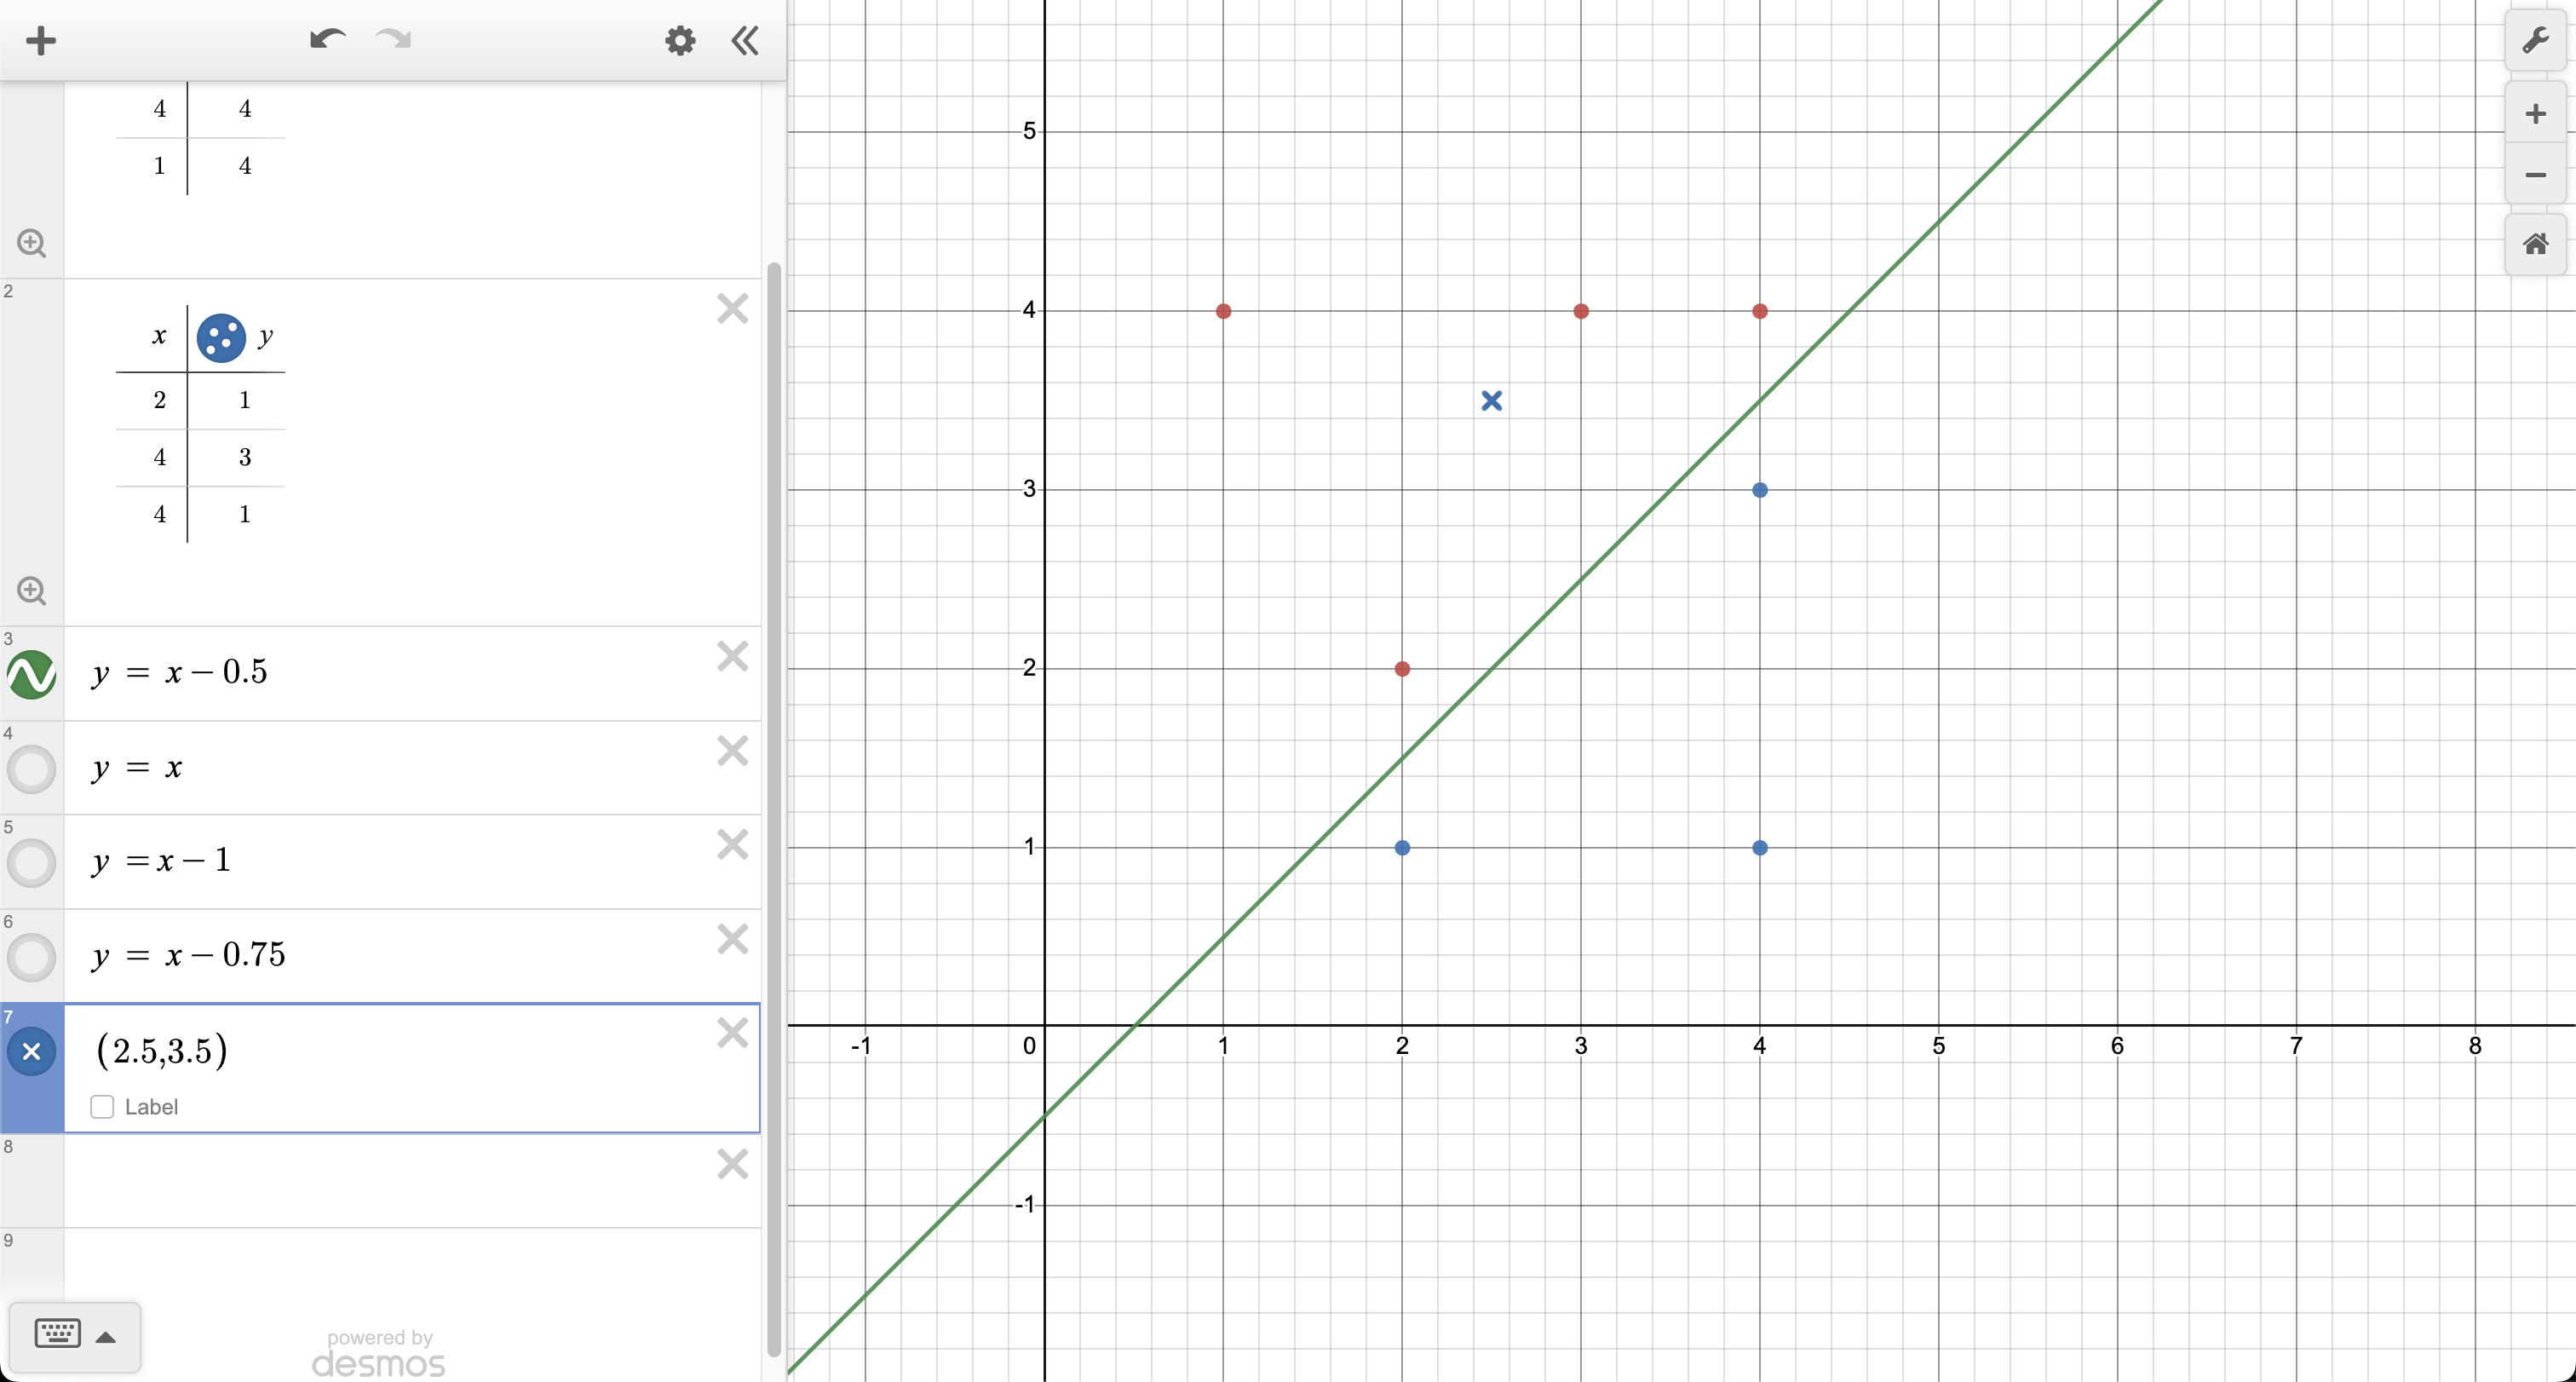
\includegraphics[width=0.5\linewidth]{HW3//images/image4.png}
    \caption{Feature Vector for Faces}
    \label{fig:enter-label}
\end{figure}

\begin{lstlisting}[language=Python]
i = 0

# Reconstruct face from the feature vector
reconstructed_face = np.dot(train_features[i, :], eigenvectors[:, :r].T) + average_face

# Display
plt.subplot(1, 2, 1)
plt.imshow(train_data_mean_subtracted[i, :].reshape(50, 50), cmap=cm.Greys_r)
plt.title("Original Face")
plt.subplot(1, 2, 2)
plt.imshow(reconstructed_face.reshape(50, 50), cmap=cm.Greys_r)
plt.title("Reconstructed Face")
plt.show()
\end{lstlisting}

\begin{figure}[H]
    \centering
    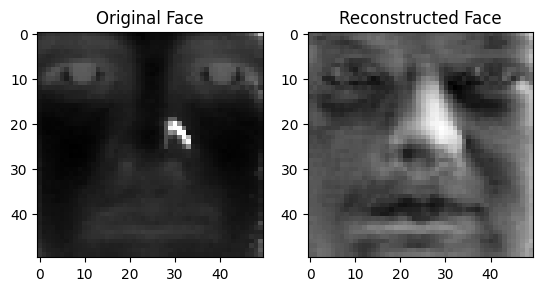
\includegraphics[width=1\linewidth]{HW3//images/image5.png}
    \caption{Reconstructed Face}
    \label{fig:enter-label}
\end{figure}

\end{Solution}

\begin{Problem*}[(g) (10 pts) Face Recognition. ]
For this problem, you are welcome to use libraries such as scikit learn to perform logistic regression. Extract training and test features for $r=10$. Train a Logistic Regression model using $\mathbf{F}$ and test on $\mathbf{F}_{\text {test }}$. Report the classification accuracy on the test set. Plot the classification accuracy on the test set as a function of $r$ when $r=1,2, \ldots, 200$. Use "one-vs-rest" logistic regression, where a classifier is trained for each possible output label. Each classifier is trained on faces with that label as positive data and all faces with other labels as negative data. sklearn calls this the "ovr" mode.
\end{Problem*}

\begin{Solution}
\begin{lstlisting}[language=Python]
from sklearn.linear_model import LogisticRegression
from sklearn.metrics import accuracy_score, f1_score, classification_report
import warnings
res = []
warnings.filterwarnings("ignore")
for r in range(1, 201):
  train_features = generate_feature_matrix(train_data_mean_subtracted, eigenvectors, r)
  test_features = generate_feature_matrix(test_data_mean_subtracted, eigenvectors, r)
  lr_model = LogisticRegression(solver='liblinear', multi_class='ovr')
  lr_model.fit(train_features, train_labels)
  test_predictions = lr_model.predict(test_features)
  accuracy = accuracy_score(test_labels, test_predictions)
  res.append(accuracy)

r_values = range(1, 201)
plt.plot(r_values, res, marker='o', linestyle='-', color='b')
plt.xlabel('r Values')
plt.ylabel('Accuracy')
plt.title('Accuracy Over Different r Values')
plt.show()
\end{lstlisting}

\begin{figure}[H]
    \centering
    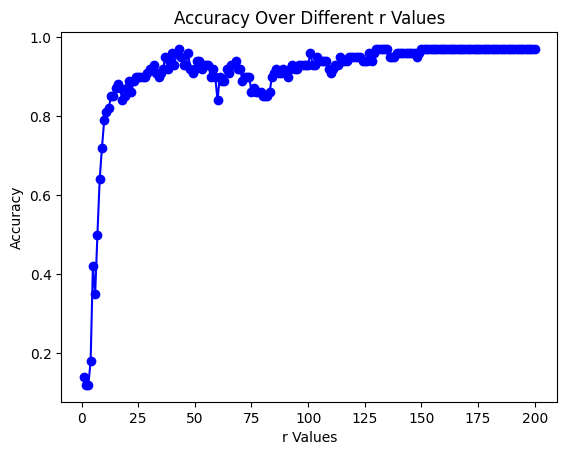
\includegraphics[width=0.5\linewidth]{HW3//images/image11.png}
    \caption{Accuracy Over Different r Values}
    \label{fig:enter-label}
\end{figure}

\end{Solution}

\begin{Problem*}[(h) (5 pts) Low-Rank Data Loss. ]
These feature matrices $\mathbf{F}$ can be mapped back to their original dimensions; however, information is lost in the process and only approximations $\mathbf{X}^{\prime}$ will be recovered. This is done by multiplying the feature matrices $\mathbf{F}$ once again by the first $r$ rows of $\mathbf{V}^{T}$. Plot the average Frobenius distance $d\left(\mathbf{X}, \mathbf{X}^{\prime}\right)=\sqrt{\operatorname{tr}\left(\left(\mathbf{X}-\mathbf{X}^{\prime}\right)^{T}\left(\mathbf{X}-\mathbf{X}^{\prime}\right)\right)}$ between the original data $\mathbf{X}$ and their approximations $\mathbf{X}^{\prime}$, over $r=1,2, \ldots, 200$.
\end{Problem*}

\begin{Solution}
\begin{lstlisting}[language=Python]
frobenius_distances = []

for r in range(1, 201):
    # Reconstruct the data using r eigenfaces
    reconstructed_data = np.dot(generate_feature_matrix(train_data_mean_subtracted, eigenvectors, r), eigenvectors[:, :r].T)
    # Compute the Frobenius distance
    difference_matrix = train_data_mean_subtracted - reconstructed_data
    distance = np.sqrt(np.trace(np.dot(difference_matrix.T, difference_matrix)))

    frobenius_distances.append(distance)

# Plot the Frobenius distances
plt.plot(range(1, 201), frobenius_distances)
plt.xlabel("Number of Eigenfaces (r)")
plt.ylabel("Frobenius Distance")
plt.title("Low-Rank Data Loss")
plt.show()
\end{lstlisting}

\begin{figure}[H]
    \centering
    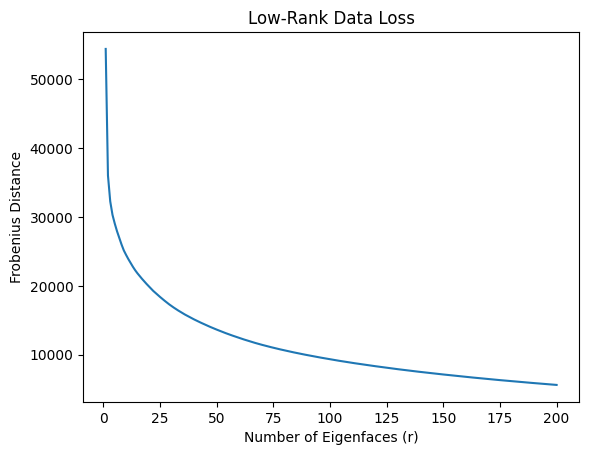
\includegraphics[width=0.5\linewidth]{HW3//images/image12.png}
    \caption{Low-Rank Data Loss}
    \label{fig:enter-label}
\end{figure}

\end{Solution}

\section{Implement EM algorithm. (40 pts)}

In this problem, you will implement a bimodal GMM model fit using the EM algorithm. Bimodal means that the distribution has two peaks, or that the data is a mixture of two groups. If you want, you can assume the covariance matrix is diagonal (i.e. it has the form $\operatorname{diag}\left(\sigma_{1}^{2}, \sigma_{2}^{2}, \ldots, \sigma_{d}^{2}\right)$ for scalars $\left.\sigma_{i}\right)$ and you can randomly initialize the parameters of the model.

You will need to use the Old Faithful Geyser Dataset. The data file contains 272 observations of the waiting time between eruptions and the duration of each eruption for the Old Faithful geyser in Yellowstone National Park.

You should do this without calling the Gaussian Mixture library in scikit learn. You can use numpy or scipy for matrix calculation or generating Gaussian distributions.


\begin{Problem*}[(a) (2 pts)]
Treat each data entry as a 2 dimensional feature vector. Parse and plot all data points on 2-D plane.
\end{Problem*}
\begin{Solution}
\begin{lstlisting}[language=Python]
import pandas as pd

data = pd.read_csv('/content/Geyser.csv')
data.drop(columns='count', inplace=True)
print(data.head())

waiting_time = data['waiting']
eruption_duration = data['eruptions']

print(waiting_time.shape, eruption_duration.shape)

plt.scatter(eruption_duration, waiting_time, c='b', marker='o', label='Data Points')
plt.xlabel('Waiting Time (minutes)')
plt.ylabel('Eruption Duration (minutes)')
plt.title('Old Faithful Geyser Data')
plt.legend()
plt.show()

\end{lstlisting}
\begin{figure}[H]
    \centering
    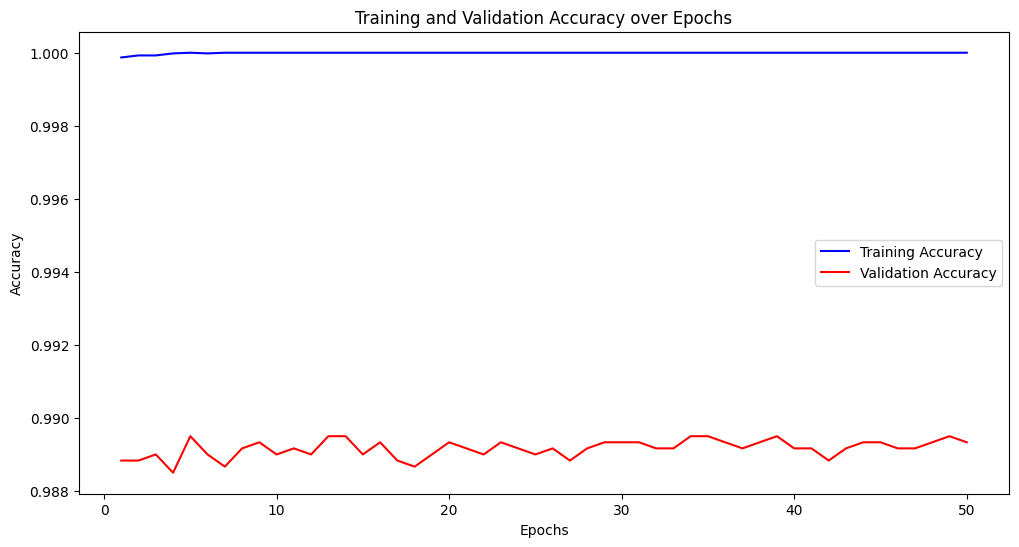
\includegraphics[width=0.5\linewidth]{HW3//images/image8.png}
    \caption{Old Faithful Geyser Data}
    \label{fig:enter-label}
\end{figure}
\end{Solution}

\begin{Problem*}[(b) (3 pts) ]
Recall that EM learns the parameter $\theta$ of a Gaussian mixture model $P_{\theta}(x, z)$ over a dataset $D=\left\{x^{(i)} \mid i=1,2, \ldots n\right\}$ by performing the E-step and the M-step for $t=0,1,2, \ldots$. We repeat the E-step and and $\mathrm{M}$-step until convergence.

In the E-step, for each $x^{(i)} \in D$, we compute a vector of probabilities $P_{\theta_{t}}(z=k \mid x)$ for the event that each $x^{(i)}$ originates from a cluster $k$ given the current set of parameters $\theta_{t}$.

Write the expression for $P_{\theta_{t}}(z=k \mid x)$, which is the posterior of each data point $x^{(i)}$. Recall that by Bayes' rule,

$$
P_{\theta_{t}}(z=k \mid x)=\frac{P_{\theta_{t}}(z=k, x)}{P_{\theta_{t}}(x)}=\frac{P_{\theta_{t}}(z=k, x)}{\sum_{l=1}^{K} P_{\theta_{t}}(x \mid z=l) P_{\theta_{t}}(z=l)} .
$$

Note that we have seen this formula in class. We are asking you to write it down and try to understand and it before implementing it in part (e).
\end{Problem*}
\begin{Solution}
Formula to use: \\
\begin{align*}
    P_\theta(z=k \mid x) &= \frac{P_\theta(z=k, x)}{P_\theta(x)}\\
    &=\frac{P_\theta(x \mid z=k) P_\theta(z=k)}{\sum_{l=1}^K P_\theta(x \mid z=l) P_\theta(z=l)}\\
    &=\frac{\mathcal{N}\left(x ; \mu_k, \Sigma_k\right) \cdot \phi_k}{\sum_{l=1}^K \mathcal{N}\left(x ; \mu_l, \Sigma_l\right) \cdot \phi_l}
\end{align*}
\end{Solution}

\begin{Problem*}[(c) (5 pts)]
In the M-step, we compute new parameters $\theta_{t+1}$. Our goal is to find $\mu_{k}, \Sigma_{k}$ and $\phi_{k}$ that optimize

$$
\max _{\theta}\left(\sum_{k=1}^{K} \sum_{x \in D} P_{\theta_{t}}\left(z_{k} \mid x\right) \log P_{\theta}\left(x \mid z_{k}\right)+\sum_{k=1}^{K} \sum_{x \in D} P_{\theta_{t}}\left(z_{k} \mid x\right) \log P_{\theta}\left(z_{k}\right)\right)
$$

Write down the formula for $\mu_{k}, \Sigma_{k}$, and for the parameters $\phi$ at the M-step (we have also seen these formulas in class).
\end{Problem*}

\begin{Solution}
Formulas for $\mu_k^*$, $\Sigma_k^*$ and $\phi_k^*$ \\
\begin{aligned}
    \mu_k^* & =\frac{\sum_{i=1}^n P\left(z=k \mid x^{(i)}\right) x^{(i)}}{n_k} \\
    \Sigma_k^* & =\frac{\sum_{i=1}^n P\left(z=k \mid x^{(i)}\right)\left(x^{(i)}-\mu_k^*\right)\left(x^{(i)}-\mu_k^*\right)^{\top}}{n_k} \\
    \phi_k^* & =\frac{n_k}{n}
\end{aligned}
\end{Solution}

\begin{Problem*}[(d)]
     Implement and run the EM algorithm.
\end{Problem*}

\begin{Problem*}[i. (10 pts)]
 Implement the EM algorithm from scratch (e.g., in Python and numpy).
\end{Problem*}
\begin{Solution}
\begin{lstlisting}[language=Python]
from scipy.stats import multivariate_normal
from sklearn.preprocessing import normalize


def e_step(X, phis, avgs, covariances):
    sampling, n_features = X.shape
    num_clusters = 2
    weights = np.zeros((sampling, num_clusters))

    for cluster in range(num_clusters):
        cluster_prior = phis[cluster]
        cluster_mean = avgs[cluster]
        cluster_covariance = covariances[cluster]
        # Create multivariate normal distribution object
        cluster_distribution = multivariate_normal(mean=cluster_mean, cov=cluster_covariance)
        # Calculate probability density using the distribution object
        pdf_values = cluster_distribution.pdf(X)
        # Calculate and store the cluster-specific weights
        cluster_weights = cluster_prior * pdf_values
        weights[:, cluster] = cluster_weights

    normalized_weights = normalize(weights, norm='l1', axis=1)
    return normalized_weights

def m_step(X, weights):
    sampling, n_features = weights.shape
    num_clusters = 2
    total_weight = weights.sum(axis=0)
    phis = total_weight / sampling
    avgs = np.zeros((num_clusters, n_features))
    covariances = np.zeros((num_clusters, n_features, n_features))

    for i in range(num_clusters):
        for j in range(n_features):
            avgs[i, j] = np.sum(weights[:, i] * X[:, j]) / total_weight[i]

    for i in range(num_clusters):
      X_centered = X - avgs[i]
      covariances[i] = np.zeros((n_features, n_features))
      for j in range(n_features):
          for k in range(n_features):
              inside_prod = weights[:, i] * X_centered[:, j]
              covariances[i][j, k] = np.sum(inside_prod * X_centered[:, k]) / total_weight[i]

    return phis, avgs, covariances

#initializations, used gpt to help generate initializations
K = 2
mu = np.random.randn(K, 2)
X = data.to_numpy()
sampling, n_features = X.shape
num_clusters = K
weights = np.zeros((sampling, num_clusters))
random_state = np.random.default_rng(seed=None)
random_indices = random_state.choice(num_clusters, sampling)
for i in range(sampling):
    weights[i, random_indices[i]] = 1

# initial M step
priors, means, covariances = m_step(X, weights)

# exit condition stated below
converged = False
means_list = []
convergence_threshold = 1e-9

while not converged:
    means_prev = means # Store the current means for comparison
    weights = e_step(X, priors, means, covariances) # Perform the E-step to update weights
    priors, means, covariances = m_step(X, weights)  # Perform the M-step to update priors, means, and covariances
    means_list.append(means) # Append the current means to the list for tracking

    #Terminal condition
    # Calculate the change in means between iterations
    mean_difference = np.sum(np.square(means_prev - means))
    converged = mean_difference < convergence_threshold

cluster_1_indices = np.where(weights[:, 0] > weights[:, 1])[0]
cluster_2_indices = np.where(weights[:, 0] <= weights[:, 1])[0]

cluster_1 = X[cluster_1_indices]
cluster_2 = X[cluster_2_indices]

mean_1, mean_2 = means_list[-1]

plt.figure(figsize=(10, 8))
plt.scatter(cluster_1[:, 0], cluster_1[:, 1], s=5, c='r', label='cluster_1')
plt.scatter(cluster_2[:, 0], cluster_2[:, 1], s=5, c='b', label='cluster_2')
plt.scatter(mean_1[0], mean_1[1], s=50, c='m', label='mean_1')
plt.scatter(mean_2[0], mean_2[1], s=50, c='g', label='mean_2')
plt.title('Clustering of Eruptions vs Waiting Time using EM Algorithm')
plt.xlabel('Eruption time in minutes')
plt.ylabel('Waiting time in minutes')
plt.legend()

plt.show()
\end{lstlisting}

\begin{figure}[H]
    \centering
    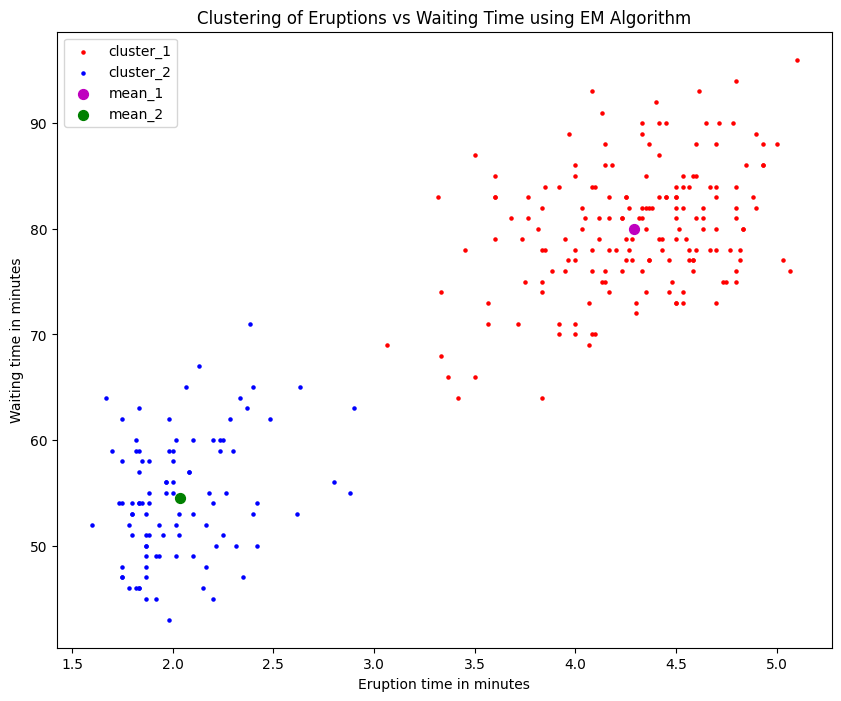
\includegraphics[width=0.5\linewidth]{HW3//images/image13.png}
    \caption{Clustering of Eruptions vs Waiting Time using EM Algorithm}
    \label{fig:enter-label}
\end{figure}

\end{Solution}

\begin{Problem*}[ii. (5 pts)]
Choose a termination criterion for when the algorithm stops repeating the E-step and the M-step. State your termination criterion and explain the reasoning behind it.
\end{Problem*}
\begin{Solution}

We chose $1e-9$ for the difference between mean and previous mean to be the the termination criterion. We believe that this difference in means would be sufficient enough to provide an accurate result. The algorithm checks this step every time until this value converges, and then we stop fitting it.

\end{Solution}

\begin{Problem*}[iii. (10 pts)]
 Plot the trajectories of the two mean vectors $\left(\mu_{1}\right.$ and $\left.\mu_{2}\right)$ in two dimensions as they change over the course of running EM. You might want to use a scatter plot for this.
\end{Problem*}
\begin{Solution}
\begin{lstlisting}[language=Python]
all_means = np.array(means_list)
mu_1, mu_2 = all_means[-1]
mu_1_hist = all_means[:, 0]
mu_2_hist = all_means[:, 1]

plt.scatter(mu_1_hist[:,0], mu_1_hist[:,1], s=4, c='b', label='cluster_1')
plt.scatter(mu_2_hist[:,0], mu_2_hist[:,1], s=4, c='r', label='cluster_2')
plt.scatter(mu_1[0], mu_1[1], s=50, c='m', label='mean_1')
plt.scatter(mu_2[0], mu_2[1], s=50, c='b', label='mean_2')
plt.xlabel('Waiting time in Minutes')
plt.ylabel('Eruption time in Minutes')
plt.title('Trajectories of Mean Vectors')
plt.legend()
plt.show()
\end{lstlisting}

\begin{figure}[H]
    \centering
    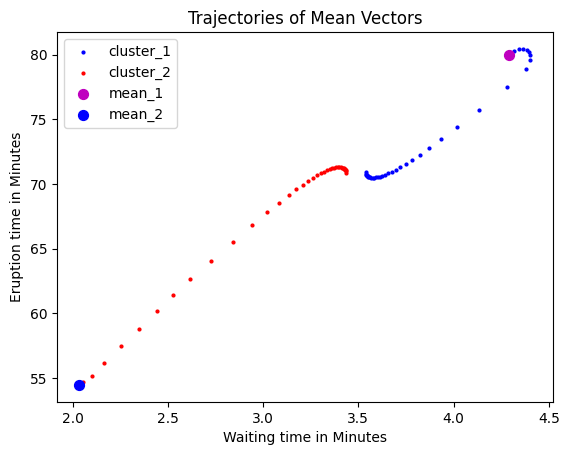
\includegraphics[width=0.5\linewidth]{HW3//images/image14.png}
    \caption{Trajectories of Mean Vectors}
    \label{fig:enter-label}
\end{figure}

\end{Solution}

\begin{Problem*}[(e) (5 pts)]
 If you were to run $K$-means clustering instead of the EM algorithm you just implemented, do you think you will get different clusters? You are welcome to experiment with $K$-means clustering on the same dataset with $K=2$. (The KNN library from scikit learn is a good way to try). Comment on why do you think the results will or will not change.
\end{Problem*}
\begin{Solution}
\begin{lstlisting}[language=Python]
from sklearn.cluster import KMeans

X = data.to_numpy()
km = KMeans(n_clusters=2, max_iter=100)
km.fit(X)
centroid1, centroid2 = km.cluster_centers_
plt.figure(figsize=(10,8))
# Scatter plot of data points
plt.scatter(X[km.labels_ == 0, 0], X[km.labels_ == 0, 1], s=4, c='r', label='Cluster 1')
plt.scatter(X[km.labels_ == 1, 0], X[km.labels_ == 1, 1], s=4, c='b', label='Cluster 1')

# Plot centroids
plt.scatter(centroid1[0], centroid1[1], c='m', marker='x', s=50, label='Centroid 1')
plt.scatter(centroid2[0], centroid2[1], c='g', marker='x', s=50, label='Centroid 2')

plt.xlabel('Waiting Time (minutes)')
plt.ylabel('Eruption Duration (minutes)')
plt.title('K-Means Clustering with Centroids')
plt.legend()
plt.show()
\end{lstlisting}

\begin{figure}[H]
    \centering
    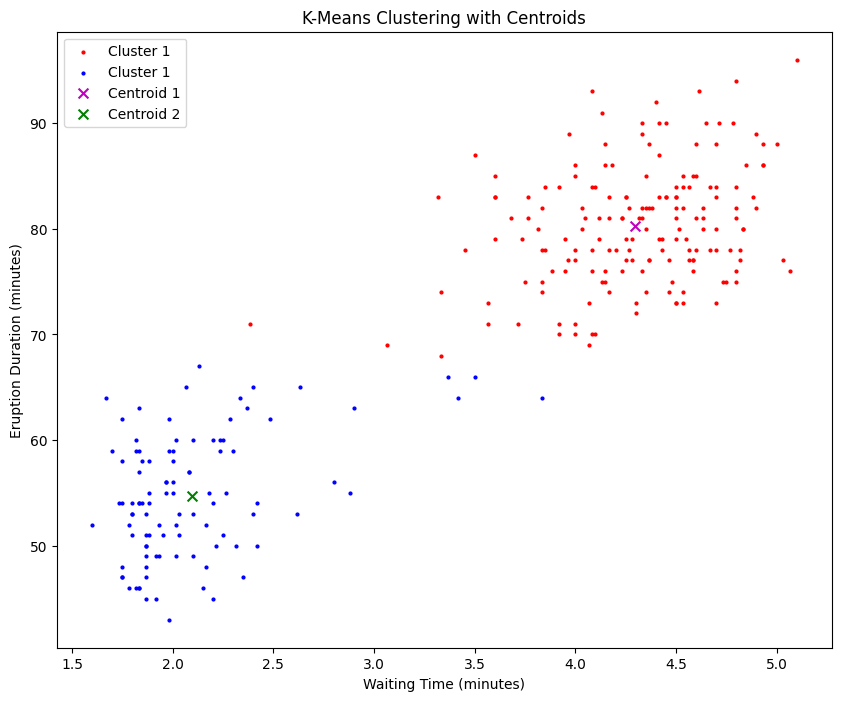
\includegraphics[width=1\linewidth]{HW3//images/image15.png}
    \caption{K-Means Clustering}
    \label{fig:enter-label}
\end{figure}

Yes, we do get different clusters. While the majority of the datapoints are clustered similarly, the way our EM implementation clustered the datapoints in the middle of the graphs was different than the way K-Means clustered them. For K-Means, the 'island' was split in two, while for the EM it was completely allocated to the first cluster.

The main reason that we believe that the clusters are different, is their objective functions. While EM maximizes the probability of the data given the model, considering Gaussian mixture components, the K-Means minimizes the sum of squared distances between data points and cluster centroids (Euclidean distance). This distinction is evident on how each algorithm handles the outliers.

\end{Solution}

\section{Kernel Density Estimation. (12pts)}
For this question, you may use existing libraries, or you may implement the method yourself in numpy. Consider the following set of $n=10$ samples drawn from a distribution.

$$
\begin{array}{llllllllll}
26 & 30 & 27 & 18 & 75 & 66 & 73 & 63 & 56 & 83
\end{array}
$$


\begin{Problem*}[(a) (4 pts)]
Let $\tilde{p}(x)=\sum_{i=1}^{n} K\left(x^{(i)}, x ; \delta\right)$ be a kernel density estimate of the data distribution with a Gaussian kernel $K(x, z ; \delta) \propto \exp \left(\frac{-\|x-z\|^{2}}{2 \delta}\right)$ and a bandwidth parameter $\delta>0$. Plot the density estimate $\tilde{p}(x)$ of the above dataset as a function of $x$ on an interval containing the data using two choices of bandwidth $\delta=100$ and $\delta=10$. For this and the rest of the problem, $\tilde{p}$ can be either a normalized or an unnormalized probability. 
\end{Problem*}
\begin{Solution}
\begin{lstlisting}[language=Python]
import numpy as np
import matplotlib.pyplot as plt
from scipy.stats import gaussian_kde
from sklearn.neighbors import KernelDensity


data = np.array([26, 30, 27, 18, 75, 66, 73, 63, 56, 83])

x_values = np.linspace(0, 100, 1000)
# Bandwidth = 100
kde100 = KernelDensity(kernel='gaussian', bandwidth=100).fit(data.reshape(-1, 1))
log_density100 = kde100.score_samples(x_values.reshape(-1, 1))
# Convert log-density estimate to probabilities
density100 = np.exp(log_density100)

# Bandwidth = 10
kde10 = KernelDensity(kernel='gaussian', bandwidth=10).fit(data.reshape(-1, 1))
log_density10 = kde10.score_samples(x_values.reshape(-1, 1))
# Convert log-density estimate to probabilities
density10 = np.exp(log_density10)

# Create subplots
fig, axs = plt.subplots(1, 2, figsize=(15, 6), sharey=True)  # 1 row, 2 columns, share y-axis

# Plot for Bandwidth = 100
axs[0].plot(x_values, density100, label=f'Bandwidth = 100')
axs[0].scatter(data, [-0.001] * len(data), c='red', marker='o', label='Data Points')
axs[0].set_xlabel('x')
axs[0].set_ylabel('Density Estimate')
axs[0].set_title('KDE with Bandwidth = 100')
axs[0].legend()
axs[0].grid()

# Plot for Bandwidth = 10
axs[1].plot(x_values, density10, label=f'Bandwidth = 10')
axs[1].scatter(data, [-0.001] * len(data), c='red', marker='o', label='Data Points')
axs[1].set_xlabel('x')
axs[1].set_ylabel('Density Estimate')
axs[1].set_title('KDE with Bandwidth = 10')
axs[1].legend()
axs[1].grid()

plt.tight_layout()
plt.show()
\end{lstlisting}

\begin{figure}[H]
    \centering
    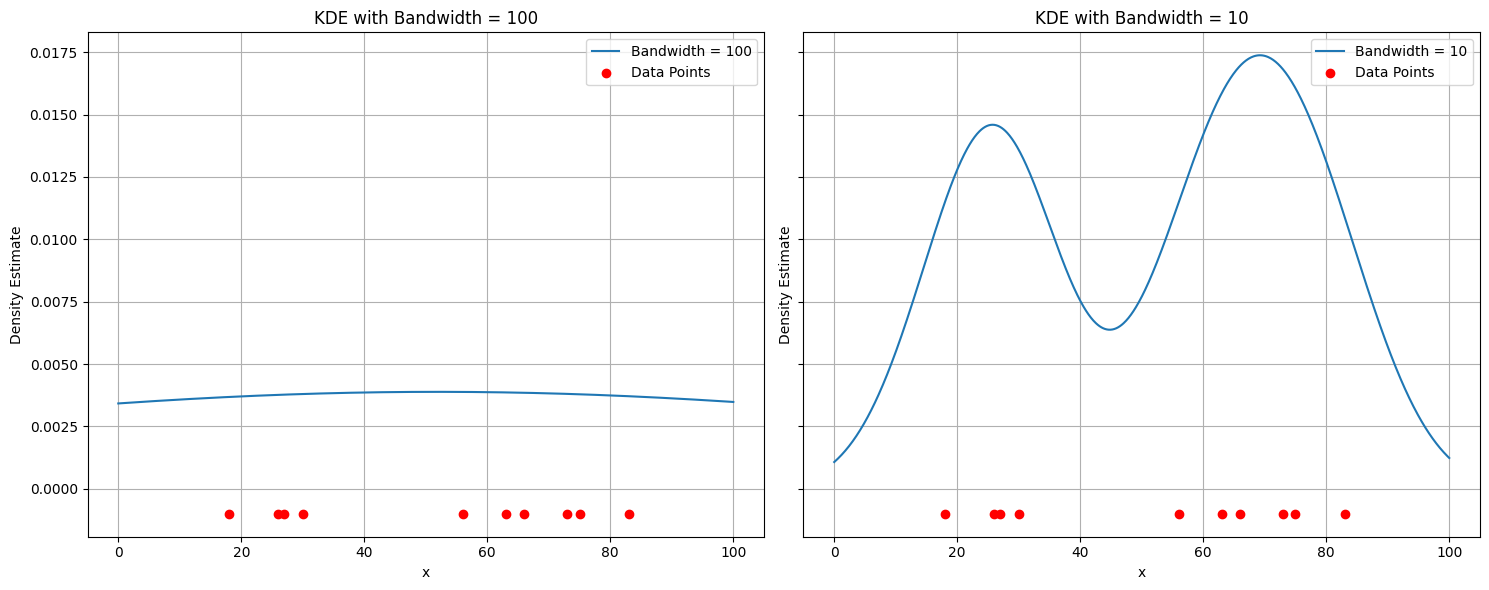
\includegraphics[width=1\linewidth]{HW3//images/image6.png}
    \caption{KDE with various bandwidths}
    \label{fig:enter-label}
\end{figure}

\end{Solution}

\begin{Problem*}[(b) (2 pts)]
 Explain which of the above two choices of $\delta$ you think is better. Name at least one method for choosing the better $\delta$ out of the two options.
\end{Problem*}
\begin{Solution}
The KDE with a bandwidth of $\delta = 10 $, captures more detailed features of the data distribution, showing peaks and valleys that align better with the location of the data points.

The choice of $\delta = 10$ seems to be better for this dataset as it captures more nuances of the data distribution. A smaller bandwidth can capture finer details of the data but can also be more susceptible to noise. A larger bandwidth, while smoothing out noise, can miss important structures in the data. Here, $\delta = 100$ seems to oversmooth the distribution.


The method we chose for picking $\delta$ is **Visual Inspection and Heuristics** 
Simply plotting the KDE for various bandwidths and choosing the one that seems to best capture the structure of the data, without being too noisy or too smooth is effective.
\end{Solution}

\begin{Problem*}[(c) (2 pts)]
 Suppose you observe two new samples: 30 and 95. Compute and report their (possibly unnormalized) probability $\tilde{p}(x)$ for both $\delta=100$ and $\delta=10$.
\end{Problem*}
\begin{Solution}
\begin{lstlisting}[language=Python]
# Function to compute the KDE for a given sample
def compute_kde(sample, data, delta):
    return np.sum(np.exp(-np.square(sample - data) / (2 * delta)))

samples = [30, 95]
deltas = [100, 10]
results = {}

for s in samples:
    for d in deltas:
        results[(s, d)] = compute_kde(s, data, d)
        print(f"Sample {s} and Delta {d}:")
        print(f"Probability = {results[(s, d)]}")
        print()
\end{lstlisting}

Sample 30 and Delta 100:
Probability = 3.405902643251741

Sample 30 and Delta 10:
Probability = 2.087703701547374

Sample 95 and Delta 100:
Probability = 0.7324039218477342

Sample 95 and Delta 10:
Probability = 0.0007465879004384897
\end{Solution}

\begin{Problem*}[(d) (2 pts)]
 Provide one possible rule by which a kernel density estimate can be used to either accept a point as being part of the data distribution or reject it for being an outlier. Provide one scenario in which this strategy might not work.
\end{Problem*}
\begin{Solution}
One possible rule to determine whether a point is part of the data distribution or an outlier using KDE is to set a threshold for the estimated density. If the estimated density for a point is below this threshold, the point can be considered an outlier. 

**Rule**: Given a threshold $T$:
- If $\tilde{p}(x) < T$ for a sample $x$, it is an outlier.
- Otherwise, it's part of the data distribution.

One scenario where this might not work is in a multimodal distribution where one mode has much lower density than the other. In such a scenario, valid data points from the lower-density mode might be mistakenly classified as outliers.
\end{Solution}

\begin{Problem*}[(e) (2 pts)]
 Let's say that instead of a Gaussian kernel, a Tophat kernel $(K(x, z ; \delta)=1$ if $\|x-z\| \leq \delta / 2$ else 0 ) is chosen for modeling. Plot the Tophat density estimate $\tilde{p}(x)$ of the dataset as a function of $x$ on an interval containing the data using $\delta=10$. Give one example of a shortcoming of the Tophat kernel density estimate for outlier detection relative to the Gaussian kernel.
\end{Problem*}
\begin{Solution}
\begin{lstlisting}[language=Python]
def tophat_kde(sample, data, delta):
    return np.sum(np.abs(sample - data) <= delta/2)

delta = 10
tophat_density = [tophat_kde(x, data, delta) for x in x_values]

plt.plot(x_values, tophat_density, label="Tophat KDE")
plt.scatter(data, [-0.5]*len(data), c='red', marker='o', label='Data Points')
plt.xlabel('x')
plt.ylabel('Density Estimate')
plt.title('Tophat KDE with Bandwidth = 10')
plt.legend()
plt.grid()
plt.show()
\end{lstlisting}

\begin{figure}[H]
    \centering
    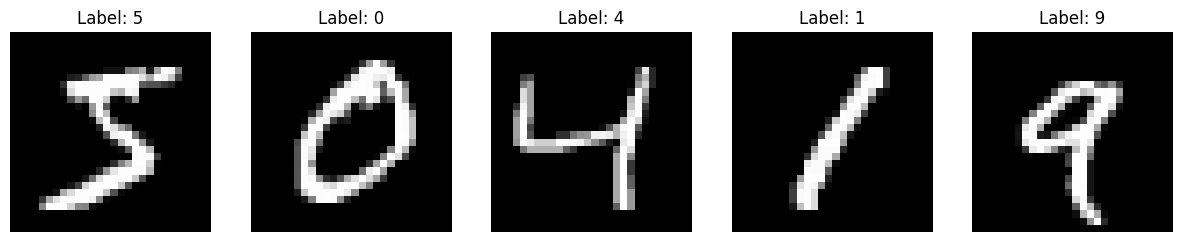
\includegraphics[width=0.5\linewidth]{HW3//images/image7.png}
    \caption{Tophat Plot}
    \label{fig:enter-label}
\end{figure}

The Tophat is less smooth and less differentiable compared to the Gaussian kernel. When used for outlier detection, the abrupt changes in the curve can result in an inability to differentiate subtle variations in the data, potentially leading to misclassifications.

\end{Solution}

\section*{Written Exercises}

\setcounter{section}{0}

\section{K-means clustering. (10 pts)}
\setcounter{Problem}{0}
K-means clustering. (10 pts) For a dataset consisting of $n$ points, $x^{(i)} \in \mathbb{R}^{d}$ for $i=1,2, \ldots n$, the goal of K-means clustering is to find a function $f: \mathbb{R}^{d} \rightarrow\{1,2, \ldots, K\}$ that assigns each point to one of $K$ clusters. Each cluster is represented by a centroid, $c^{(k)} \in \mathbb{R}^{d}$ for $k=1,2, \ldots, K$. Recall from the lecture on unsupervised learning that the K-means objective is optimized by an iterative process. For each iteration $t$, let $f_{t}$ denote the cluster assignment function and $c_{t}^{(k)}$ denote the $k^{\text {th }}$ centroid. Then, at each iteration $t$, we perform two steps: (1) update cluster assignments $f_{t}\left(x^{(i)}\right)$ for each point $x^{(i)}$ and (2) update centroids $c_{t}^{(k)}$ for each cluster $k=1,2, \ldots, K$ :

Initialization: set centroids $c_{0}^{(k)}$ randomly or using an initialization heuristic. For $t=1,2, \ldots$ until K-Means converges, do:

\begin{enumerate}
    \item[Step 1.] Update cluster assignments such that $f_{t}\left(x^{(i)}\right)=\operatorname{argmin}_{k}\left\|x^{(i)}-c_{t-1}^{(k)}\right\|_{2}$ is the cluster of the closest centroid to $x^{(i)}$, where $\|\cdot\|_{2}$ denotes Euclidean norm.

    \item[Step 2.] Set each centroid $c_{t}^{(k)}$ to be the average of its cluster. Letting $S^{(k)}=\left|\left\{x^{(i)} \mid f_{t}\left(x^{(i)}\right)=k\right\}\right|$ be the number of points assigned to cluster $k$, we refit centroids as follows:

$$
c_{t}^{(k)}=\frac{1}{S^{(k)}} \sum_{i: f_{t}\left(x^{(i)}\right)=k} x^{(i)}
$$
\end{enumerate}

Letting $c_{t}$ (i.e., without any superscript) be a shorthand representation for all $K$ centroids $\left\{c_{t}^{(1)}, c_{t}^{(2)}, \ldots, c_{t}^{(K)}\right\}$, we can express the K-means optimization objective at each time $t$ as follows:

$$
J\left(c_{t}, f_{t}\right)=\sum_{i=1}^{n}\left\|x^{(i)}-c_{t}^{\left(f_{t}\left(x^{(i)}\right)\right)}\right\|_{2}
$$

where $c_{t}^{\left(f_{t}\left(x^{(i)}\right)\right)}$ denotes "the centroid for the cluster assignment of $x^{(i)}$ at time $t$ ". In this question, we want to prove that K-means optimization is guaranteed to converge. In other words, we want to prove that the K-means objective $J\left(c_{t}, f_{t}\right)$ is monotonically decreasing after each step of K-means optimization procedure:

$$
J\left(c_{t}, f_{t}\right) \leq J\left(c_{t-1}, f_{t-1}\right)
$$

If we prove this, then convergence follows from the monotone convergence theorem, which states that a monotonically decreasing sequence with a lower bound (the bound is $J\left(c_{t}, f_{t}\right) \geq 0, \forall t$, in our case) is guaranteed to converge.

\begin{Problem*}[(a) (5 pts)]
 Show that $J\left(c_{t-1}, f_{t}\right) \leq J\left(c_{t-1}, f_{t-1}\right)$. This is equivalent to proving that the K-means objective is decreasing after updating cluster assignments (but before updating the centroids).
\end{Problem*}
\begin{Solution}
To show that the K-means objective \( J(c_{t-1}, f_t) \) is no larger than \( J(c_{t-1}, f_{t-1}) \) after the cluster assignment update, we'll need to analyze how the cluster assignments are updated.

Given:
\[ J\left(c, f\right)=\sum_{i=1}^{n}\left\|x^{(i)}-c^{\left(f\left(x^{(i)}\right)\right)}\right\|_{2} \]
\[ f_t(x^{(i)}) = \operatorname{argmin}_k \left\| x^{(i)} - c_{t-1}^{(k)} \right\|_2 \]

Now, for a specific data point \( x^{(i)} \):

\[ J\left(c_{t-1}, f_{t-1}\right)_i = \left\| x^{(i)} - c_{t-1}^{f_{t-1}(x^{(i)})} \right\|_2 \]
\[ J\left(c_{t-1}, f_t\right)_i = \left\| x^{(i)} - c_{t-1}^{f_t(x^{(i)})} \right\|_2 \]

Given the definition of \( f_t \), we know:
\[ f_t(x^{(i)}) = \operatorname{argmin}_k \left\| x^{(i)} - c_{t-1}^{(k)} \right\|_2 \]

This means the term \( \left\| x^{(i)} - c_{t-1}^{f_t(x^{(i)})} \right\|_2 \) is the smallest possible Euclidean distance from \( x^{(i)} \) to any of the centroids from the previous iteration. 

Assume that there is a Euclidean distance $a$ that we obtained from $J\left(c_{t-1}, f_t\right)_i$. And also a Euclidean distance $b$ that we obtained from $J\left(c_{t-1}, f_{t-1}\right)_i$, which is greater than $a$. Considering that inherent nature of the $\operatorname{argmin}$ function is to either to update to smaller value or at worst, keep the value the same, it is impossible for $b$ to be greater than $a$.

Thus:
\[ J\left(c_{t-1}, f_t\right)_i \leq J\left(c_{t-1}, f_{t-1}\right)_i \]

Since the above inequality holds for every \( i \) from 1 to \( n \), summing over all \( n \) data points, we get:
\[ J\left(c_{t-1}, f_t\right) \leq J\left(c_{t-1}, f_{t-1}\right) \]

This proves that the K-means objective function does not increase after updating the cluster assignments, keeping the centroids the same. In other words, reassigning points to the nearest centroid can only decrease (or at worst, keep the same) the sum of the squared distances.


\end{Solution}

\begin{Problem*}[(b) (5 pts)]
 Show that $J\left(c_{t}, f_{t}\right) \leq J\left(c_{t-1}, f_{t}\right)$. This is equivalent to proving that the K-means objective is decreasing after refitting centroids.
\end{Problem*}

\begin{Solution}
For each cluster \( k \), the cost incurred by the data points assigned to it is:

\[ \sum_{i: f_t\left(x^{(i)}\right) = k} \left\| x^{(i)} - c \right\|_2^2 \]

The cost for centroids \( c_t^{(k)} \) and \( c_{t-1}^{(k)} \):

Cost for \( c_t^{(k)} \):
\[ \sum_{i: f_t\left(x^{(i)}\right) = k} \left\| x^{(i)} - c_t^{(k)} \right\|_2^2 \]

Cost for \( c_{t-1}^{(k)} \):
\[ \sum_{i: f_t\left(x^{(i)}\right) = k} \left\| x^{(i)} - c_{t-1}^{(k)} \right\|_2^2 \]

Given the definition of \( c_t^{(k)} \), we know that it's the mean of all the points assigned to cluster \( k \). This implies that \( c_t^{(k)} \) minimizes the sum of squared distances from all the points assigned to cluster \( k \). Therefore, for each cluster \( k \):

\[ \sum_{i: f_t\left(x^{(i)}\right) = k} \left\| x^{(i)} - c_t^{(k)} \right\|_2^2 \leq \sum_{i: f_t\left(x^{(i)}\right) = k} \left\| x^{(i)} - c_{t-1}^{(k)} \right\|_2^2 \]

This inequality suggests that for each cluster \( k \), the cost with the new centroid \( c_t^{(k)} \) is no larger than the cost with the previous centroid \( c_{t-1}^{(k)} \).

By summing the cost over all clusters from 1 to \( K \), we obtain:
\[ J\left(c_t, f_t\right) \leq J\left(c_{t-1}, f_t\right) \]

This proves that the K-means objective function does not increase after refitting the centroids while keeping the cluster assignments the same. In other words, moving the centroid to the mean of its assigned points can only decrease (or at worst, keep the same) the sum of the squared distances.
\end{Solution}

\section{Local Optima in K-means.}
\begin{Problem*}[(5pts)]
 Depending on initialization, K-means can get stuck on local optima. Construct an example dataset ( $>3$ points), and provide two different initializations for it such that K-means would return different final clusterings on it.
\end{Problem*} 

\begin{Solution}
Here's an example dataset consisting of 6 data points:

\[ D = \{1, 3, 5, 10, 12, 14\} \]

Now, imagine we want to cluster these into 2 clusters using K-means.

Initialization 1:  \\
Let's use two centroids initialized at:  
\[ c_1 = 2 \]  
\[ c_2 = 11 \]

In the first iteration:  
- Points \(1\), \(3\), and \(5\) would be assigned to \(c_1\).
- Points \(10\), \(12\), and \(14\) would be assigned to \(c_2\).

After refitting the centroids:  
\[ c_1' = \frac{1+3+5}{3} = 3 \]
\[ c_2' = \frac{10+12+14}{3} = 12 \]

The centroids have shifted, but the assignments will remain the same in the subsequent iteration since no point is closer to a different centroid. Thus, K-means will converge with clusters:  
\[ \{1, 3, 5\} \]
\[ \{10, 12, 14\} \]

Initialization 2: \\
Assume different initializations:  
\[ c_1 = 4 \]  
\[ c_2 = 6 \]

In the first iteration:  
- Points \(1\), \(3\), and \(5\) would be assigned to \(c_1\).
- Points \(10\), \(12\), and \(14\) would be assigned to \(c_2\).

However, when you refit the centroids:
\[ c_1' = \frac{1+3+5}{3} = 3 \]
\[ c_2' = \frac{5+10}{2} = 7.5 \]

In the next iteration:
- Points \(1\), \(3\), and \(5\) would still be assigned to \(c_1'\).
- But now, points \(10\) and \(12\) are closer to \(c_2'\), and \(14\) is equidistant. Depending on the implementation of K-means, \(14\) could be assigned to either centroid, but for this example, let's say it's assigned to \(c_2'\).

Refitting the centroids again:
\[ c_1'' = 3 \] (unchanged)
\[ c_2'' = \frac{10+12+14}{3} = 12 \] (back to the earlier position)

Now, the algorithm will oscillate between these states and might not converge depending on the implementation. However, in implementations that check for no change in the cluster assignment, it will converge when centroids don't change any further. For this example, we'll end up with clusters:
\[ \{1, 3, 5\} \]
\[ \{10, 12, 14\} \]

In this case, despite different initializations, the final clusters are the same due to the nature of the data and initializations chosen. However, with more complex and high-dimensional datasets, different initializations can indeed lead to different final clusters due to local optima.
\end{Solution}

%%%%%%%%%%%%%%%%%%%%%%%%%%%%%%%%%%%%%%%%%%%%%%%%%%%%%%%%%%%%%%%%%%
%Complete the assignment now
\end{document}

%%%%%%%%%%%%%%%%%%%%%%%%%%%%%%%%%%%%%%%%%%%%%%%%%%%%%%%%%%%%%%%%%%
%%%%%%%%%%%%%%%%%%%%%%%%%%%%%%%%%%%%%%%%%%%%%%%%%%%%%%%%%%%%%%%%%%
